%! Author = Charles Yang

% Preamble
\documentclass[11pt]{article}

% Packages
\usepackage{amsmath}
\usepackage{amsfonts}
\usepackage{hyperref}
\usepackage{enumitem}
\usepackage{graphicx}

% Settings
\setlist[enumerate]{font=\bfseries}

% Title Info
\title{STAT 347 HW6}
\author{Charles Yang}

\addtolength{\oddsidemargin}{-.875in}
\addtolength{\evensidemargin}{-.875in}
\addtolength{\textwidth}{1.75in}
\addtolength{\topmargin}{-.875in}
\addtolength{\textheight}{1.75in}

% Document
\begin{document}
    \maketitle

    \begin{enumerate}
        \item[4.42] $\frac{\theta_1 + \theta_2}{2}$

        \item[4.43] $E(A) = E(\pi r^2) = \pi E(r^2) = \pi \int_0^1 r^2 dr = \frac{\pi}{3}$

        \item[4.58]
        \begin{enumerate}
            \item[a] $0.54776 - 0.5 = 0.04776$
            \item[b] $0.5 - 0.46414 = 0.03586$
            \item[c] $0.94062 - 0.61791 = 0.32271$
        \end{enumerate} 

        \item[4.59]
        \begin{enumerate}
            \item[a] $0$
            \item[b] $1.10$
            \item[c] $1.64$
            \item[c] $2.58$
        \end{enumerate} 

        \item[4.71]
        \begin{enumerate}
            \item[a] $(0.12 - 0.13)/0.005 = -2.00$, $P(-2 < Z < 2) = 0.9545$
            \item[b] $0.9545^4 = 0.8300$
        \end{enumerate}

        \item[4.89] $\beta = \frac{1}{\lambda}$
        \begin{enumerate}
            \item[a] $P(Y > 2) = \int_2^{\infty} \frac{1}{\beta} e^{\frac{-x}{\beta}} dx = -e^{\frac{-x}{\beta}} |_2^{\infty} = e^{-\frac{2}{\beta}} = 0.0821 \implies \beta = 0.8 = E(Y)$
            \item[b] $\lambda = \frac{1}{0.8} = 1.25$, $P(Y < 1.7) = \int_0^{1.7} 1.25e^{-1.25x} dx = -e^{-1.25x} |_0^{1.7} = 0.8806$
        \end{enumerate}

        \item[4.126]
        \begin{enumerate}
            \item[a] $\int_0^y 6t-6t^2 dt = 3t^2 - 2t^3 |_0^y = 3y^2 - 2y^3$ for $y \in [0,1]$, $0$ for $y < 0$, $1$ for $y > 1$
            \item[b] 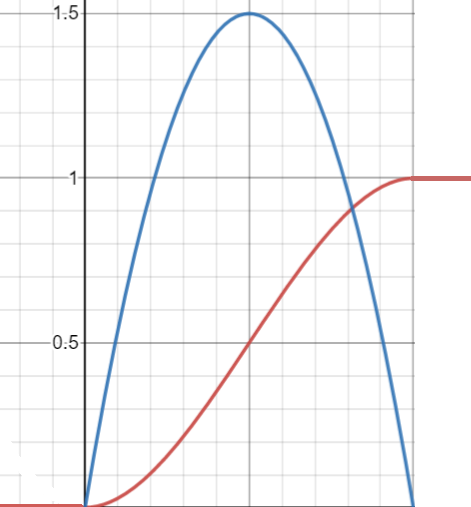
\includegraphics{4.126.b.PNG}
            \item[c] $F(0.8) - F(0.5) = 0.896 - 0.5 = 0.396$
        \end{enumerate}

        \item[4.144]
        \begin{enumerate}
            \item[a] This is the standard normal distribution. $k = \frac{1}{\sqrt{2\pi}}$
            \item[b]
            \begin{align*}
                m_y(t) = E(e^{tY}) &= \frac{1}{\sqrt{2\pi}} \int_{-\infty}^{\infty} e^{yt} e^{\frac{-y^2}{2}} dy \\
                &= \int_{-\infty}^{\infty} e^{\frac{-y^2}{2} + yt} dy \\
                &= \int_{-\infty}^{\infty} e^{\frac{-y^2}{2} + yt - \frac{t^2}{2} + \frac{t^2}{2}} dy \\
                &= \int_{-\infty}^{\infty} e^{\frac{1}{2}(z - t)^2} e^{\frac{t^2}{2}} dy \\
                &= e^{\frac{t^2}{2}} \int_{-\infty}^{\infty} e^{\frac{1}{2}(z - t)^2} dy \\
                &= e^{\frac{t^2}{2}} (1)
            \end{align*}
            \item[c] Since this is standard normal, mean is 0 and variance is 1.
        \end{enumerate}   
    \end{enumerate}


\end{document}